\documentclass{aastex62}

\newcommand{\vdag}{(v)^\dagger}
\newcommand\aastex{AAS\TeX}
\newcommand\latex{La\TeX}

%% Tells LaTeX to search for image files in the 
%% current directory as well as in the figures/ folder.
\graphicspath{{./}{figures/}}


%% Reintroduced the \received and \accepted commands from AASTeX v5.2
\received{October 1, 2018}
\revised{---}
\accepted{---}
%% Command to document which AAS Journal the manuscript was submitted to.
%% Adds "Submitted to " the arguement.
\submitjournal{ApJ}

\shorttitle{Alternative Theories}
\shortauthors{Kavelaars et al.}

\watermark{NRC-DRAFT}

\begin{document}

\title{Perspectives on the distribution of orbits of distant Trans-Neptunian Objects}

\correspondingauthor{J. J. Kavelaars}
\email{JJKavelaars@gmail.com}
\author[0000-0001-7032-5255]{J. J. Kavelaars}
\affil{Department of Physics and Astronomy, University of Victoria, Elliott Building, 3800 Finnerty Rd, Victoria, BC V8P 5C2, Canada}
\affil{Herzberg Astronomy and Astrophysics Research Centre, National Research Council of Canada, 5071 West Saanich Rd, Victoria, British Columbia V9E 2E7, Canada}


\author[0000-0001-5368-386X]{Samantha M. Lawler}
\affiliation{NRC-Herzberg Astronomy and Astrophysics, National Research Council of Canada, 5071 West Saanich Rd, Victoria, British Columbia V9E 2E7, Canada}

\author[0000-0003-3257-4490]{Michele T. Bannister}
\affiliation{Astrophysics Research Centre, School of Mathematics and Physics, Queen's University Belfast, Belfast BT7 1NN, United Kingdom}

\author[0000-0002-3507-5964]{Cory Shankman}
\affiliation{Department of Physics and Astronomy, University of Victoria, Elliott Building, 3800 Finnerty Rd, Victoria, BC V8P 5C2, Canada}


\begin{abstract}

Hello, that was abstract. 

\end{abstract}

%% Keywords should appear after the \end{abstract} command. 
%% See the online documentation for the full list of available subject
%% keywords and the rules for their use.
\keywords{Kuiper belt, orbits --- biases ---  surveys}

%% From the front matter, we move on to the body of the paper.
%% Sections are demarcated by \section and \subsection, respectively.
%% Observe the use of the LaTeX \label
%% command after the \subsection to give a symbolic KEY to the
%% subsection for cross-referencing in a \ref command.
%% You can use LaTeX's \ref and \label commands to keep track of
%% cross-references to sections, equations, tables, and figures.
%% That way, if you change the order of any elements, LaTeX will
%% automatically renumber them.
%%
%% We recommend that authors also use the natbib \citep
%% and \citet commands to identify citations.  The citations are
%% tied to the reference list via symbolic KEYs. The KEY corresponds
%% to the KEY in the \bibitem in the reference list below. 

\section{Introduction}

Looking at the orbits of planets at large-a we are compelled to see patterns. Some of those patterns are noted as indicators of strong indicators or new or hidden processes in the outer solar system, others are substantially observational biases, and still others are completely overlooked. We can gain insight into the current and past structure of the outer solar system through a careful examination of these orbital parameters. 

In this chapter we discuss the implications that can be taken from the observed distant TNO orbital distribution.  We start with some cautions on observational biases inherent in the population of known TNOs.  Some of these biases are intrinsic the process of discovery TNOs while others can be reduced or eliminated through careful survey design. We then discuss some orbital element correlations that have received considerable attention in the recent literature. We then examine the known objects in the context of the physical processes known to be at play in the Kuiper belt.  We then discuss proposed new elements to the outer solar system and posited ancient processes and the types of orbital element distributions they predict to exist.  We conclude with speculation.

\section{Biases in detection of distant solar system objects.}

We perceive the reality of the universe through our observation of that universe and our understanding of those observations are biased by our observation and perception biases. This truism of observational science must be kept in mind when considering the review of our data. As a group we examine data and look for meaning in the correlations between quantities and strongly cling to our initial conceptions.  To see beyond our perception biases is difficult and perhaps intractable. 

The Kuiper belt is over 4.5 billion km distant from the Earth bound observer with the most distant objects known three times further away still.  The challenge of detecting objects at these great distances should not be under-estimated.  Sun's like is dimmed by $r^4$, greatly exaggerating our sensitivity to nearby sources in comparison to more distant objects.  The volume of the solar neighbourhood that a survey is sensitive to, its {\it detection volume}  is, at minimum, limited in radial extent. The strength of the $r^4$ observational bias is frequently under appreciated when attempting to interpret the distributions of objects detected by a particular survey.

Objects on orbits with moderate to large eccentricities also present a distorted view of population.  Those objects occupy a range of solar distances, resulting in a time variable $r^4$-flux bias. An object may only spend a small fraction of its orbital period within the detection volume of a particular survey. The larger the semi-major axis, the larger the eccentricity needed to bring the object within the detection volume and the smaller the fraction of the orbit that object remains in that volume of space.

Limited telescopic resources add another layer of complexity to the problem of seeing the biases inherent in the detected sample.  Essentially, one can only detect objects in the part of the sky where one looks.  This observer direction bias imposes a relation between the Nodal angle, argument of peri-centre, mean anomaly and inclination of an orbit that can be detected.  This coupling of multiple angles can be difficult to conceptualize.  For illustration, we consider a discovery survey whose fields all straddle the ecliptic plane.  In those surveys,  orbits that are inclined to the ecliptic plane will have an inclination that is larger than the field of the camera will only be visible 

In Figure~1 we present the orbital distribution of a subsample of objects reported to the Minor Planet Centre. This figure presents all objects (dots) with $a > 150$~au and $q > 30$~au.  The vertical line at 1000~au {\em roughly} separates that part of the phase space where galactic and stellar passages become important. The horizontal dash line indicates the zone below which outward diffusion from the Kuiper belt is significant while the dot-dashed line indicates the zone where inward diffusion from the inner Oort cloud occurs \citep[see][for details]{bannister17}.  Also shown in this figure is a rough guide of the size of population needed to detect an object in a given ($a,q$) orbit for a survey that detected one object with $a = 150$~au and $q = 30$~au (assuming a size-frequency distribution  $ \Sigma{N} = 10^{0.5*(H-H_o)}$).  From this figure we can see that the lack of detections of $q>60$~au, $a > 1000$~au is not a strong constraint on the size of that population. One would require 220 such objects to exist in such orbits before a survey that detected one object the inner edge would expect to have one such detection.  We would need 100s of detections in the low-a/q zone just to rule out a uniform distribution in this phase-space.  These numbers are in basic agreement with more careful computation provided else where and are given here to guide the reader's understanding of the influence of orbit and flux bias in the detected sample.

An important consideration here is that to use the biases in Figure~1 to aid in understanding the structure of the trans-neptune region we need to know the full range of orbits including those with $a< 200$ and $q<40$ as we can then use the relative sensitivity to scale between the regions. 

One point that is work noting here is the lack of detections in the region showing by the hashed box in Figure~1.  The hashed box region is devoid of known objects but, generally, our sensitivity to orbits in this zone is not lower than that of other zones where a number of detections are available.  This likely indicates that this zone is, indeed, relatively under-populated, an important point in constraining the dynamics of this region of the solar system.

\begin{figure}
\centering
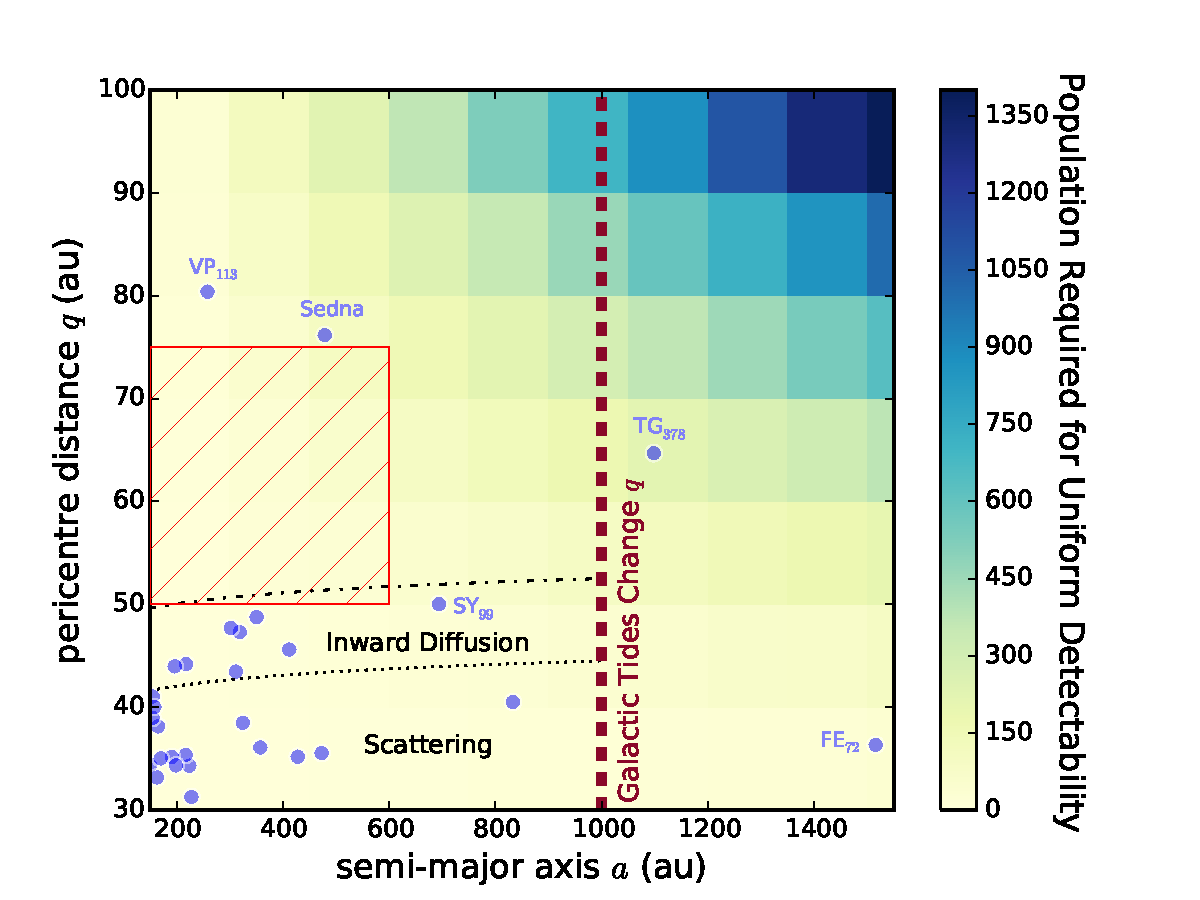
\includegraphics[width=\textwidth]{figure1.pdf}
\caption{Distribution of known TNOs (observed arcs longer than 10 months) with $a > 150$ and $q > 30$ in $a$-$q$ (blue dots).  Also shown are the approximate $q$ boundary below which inward diffusion from the $a > 1000$-au (solid vertical line)  is significant and the $q$ boundary below which outward diffusion in $a$ is significant. The grid of numbers indicates the number of objects needed in each orbit group for detection of that orbit to have similar probability to an orbits with $a = 150$, $q = 30$, see text for details.}
\label{fig:bias}
\end{figure}

\section{Diffusion and motion of large semi-major axes orbits}

\section{Biases in the angle of pericentre detection in the large-q large-a TNO sample}

Much has been made of the alignment of the pericentre angle of TNOs with $a>150$~au.  In Figure~2 we present the current sample of such orbits (as of 1-Oct-2018) to allow some examination of that sample.  The figure presents the sample of 6 orbits that created the original speculation (blue points) and the next six objects detected (orange points) and then the remaining current sample in green.  The feature that drew the attention of the discovers was the lack of detection of objects with $250< \omega < 60$.  Flux bias in the detected sample causes most detections to be of objects near the pericentres of the orbits (ie. with Mean Anomally (M) near 0 or 360).   Coupled with the habit of conducting TNO searches in fields that are predominantly straddle the sky location of the heliocentric plane forces most discovered objects to have values of $\omega$ near 0 (or 360) and 180.  Although the preference for angles near 360 is clearly present in the early sample, there were no detections found near 180.  A puzzling feature in the sample.

In the same figure we give, on a grid of locations, the relative number of detections one might expect at the given locations $\Omega$, $\omega$ values when drawing from a sample that is uniformly distributed but with $a$, $q$, $i$ sampled from the known objects and assuming a flux-limited survey focussing on fields south of the ecliptic and observing in September, October, November and February and March.  From the grid of numbers we can see that there are parts of the $\Omega$, $\omega$ space that are strongly preferred.  Our example survey is just provided as thought experiment to alert the reader to the complexity of the bias interactions. The alignment first reported is now, largely, washed out by the increased sample size but there continues to be a paucity of detections near $\omega = 180$.  Without detailed knowledge of the pointing history and careful measuring of a survey's detection and tracking efficiency, interpretation of Figure~2 is problematic at best.   Regardless of this distributions physical reality, there are no described gravitational processes that  kept $\omega$ values away form 180 degrees and accepting that the distribution is most likely observational biases is the only supportable explanation.

Subsequent to the claim of an alignment of $\omega$ values, possible alignment in the longitude of pericentre ($\tilde{\omega}$) has become a popular point of discourse.  The appeal being that one can conceive of physical processes that might align the values of $\tilde{\omega}$, making this a plausibly physical structure.  However, one must consider that the false alignment that exists within the $\omega$ propagates forward into a clustering $\tilde{\omega}$ as the values of $\Omega$ are not uncorrelated (see Figure~2).  Thus, although there are good physical mechanism to cause a clustering or alignment of  $\tilde{\omega}$ the clustering of the observed values of $\tilde{\omega}$ is driven by the same observational biases reported in the previous paragraph.

\begin{figure}
\centering
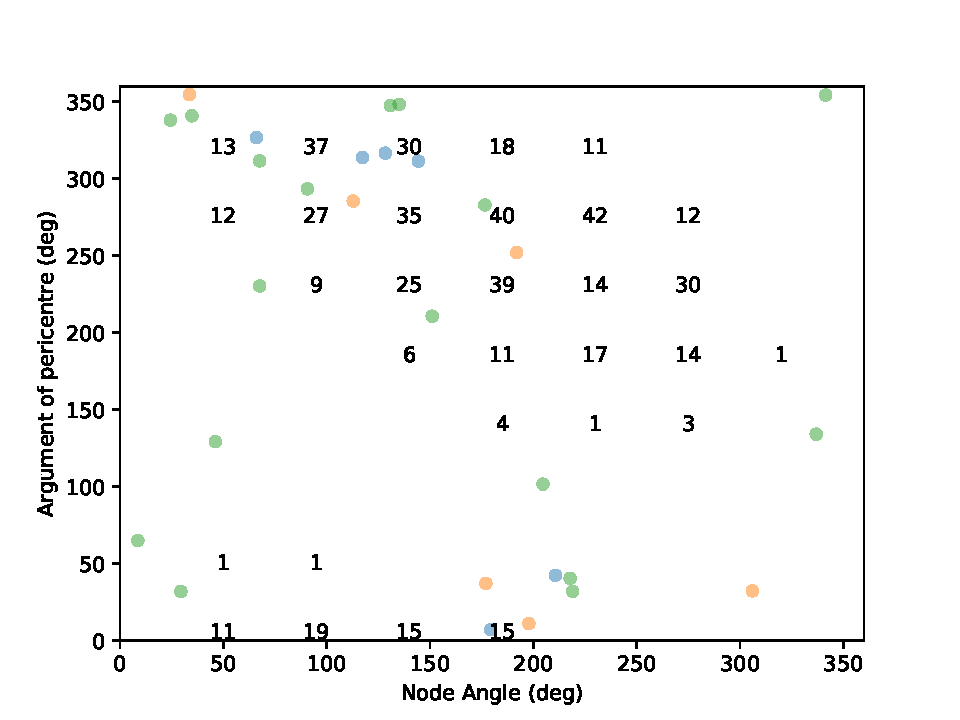
\includegraphics[width=\textwidth]{figure2.pdf}
\caption{Distribution of known TNOs (observed arcs longer than 10 months) with $a > 150$ and $q > 30$ in $\Omega$-$\omega$.  Blue dots indicate the first six such known objects, orange dots the next six and the green dots the remaining sample.  The lack of objects with values of $\omega$ near 180 degrees is not an easy bias to disentangle.  The grid of numbers indicate the number of objects a mock survey would have detected on a gird of $\Omega$, $\omega$ values (grid locations without a number had zero (0) detections.  See text for details.}
\label{fig:bias}
\end{figure}

\section{Dynamical effects expected to be imprinted on the distant Kuiper belt by the presence of a massive planet}

The authors of this chapter have already reported some of the problematic orbital evolution effects that a additional massive planet in the outer solar system would create.  In  those works we find that the alignment of orbits is caused by a massive external planet are is particularly strong \citep{shankman17}  and the signature of such an alignment would be difficult to detect in the current sample \citep{lawler17}.  Thus, our expectation is that this process is not at work and there is not strong evidence of a massive external perturber.

Figure~1, however, provides an intriguing possibility.  We may, in fact, be able to exclude the existence of such a planet. From the figure one can see that there are no objects with peri-centres between 50 and 80 au.  Indeed, other authors have already remarked on the absence of such orbits.  Recall that in Figure~1 the grid of numbers provides some measure of the inverse probability of detection of particular obits, given a survey.  A survey that might have detected an object at $a \sim 500$ and $q \sim75$ is actually more likely to have detected objects wth similar $a$ but smaller values of $q$, the same is true of the any other $q$ > 70 detections, the lower-$q$ but similar $a$ detections are always more likely.  Thus, the lack of detections in the $50 < q < 70$~au range indicates that there really are not objects in this range.  This strongly contradicts models of orbital evolution that include a massive external planet as the gravitational action of such a object invariable drags many objects from below and above this zone into it.  Thus, if the lack of objects in this q-zone is real, and currently the evidence suggests that it is, then the hypothesized external planet can be excluded\footnote{there may be some very specialized orbital configuration that preserves the emptiness of this  $q$ zone but, as of this writing, none have been proposed}.


\section{Conclusion: The orbits of Sedna and 2012 VP112 are weird.}


% \bibliographystyle{apj}
\bibliography{citations}

%% This command is needed to show the entire author+affilation list when
%% the collaboration and author truncation commands are used.  It has to
%% go at the end of the manuscript.
%\allauthors

%% Include this line if you are using the \added, \replaced, \deleted
%% commands to see a summary list of all changes at the end of the article.
%\listofchanges

\end{document}

% End of file `sample62.tex'.
